% This is "sig-alternate.tex" V2.0 May 2012
% This file should be compiled with V2.5 of "sig-alternate.cls" May 2012
%
% This example file demonstrates the use of the 'sig-alternate.cls'
% V2.5 LaTeX2e document class file. It is for those submitting
% articles to ACM Conference Proceedings WHO DO NOT WISH TO
% STRICTLY ADHERE TO THE SIGS (PUBS-BOARD-ENDORSED) STYLE.
% The 'sig-alternate.cls' file will produce a similar-looking,
% albeit, 'tighter' paper resulting in, invariably, fewer pages.
%
% ----------------------------------------------------------------------------------------------------------------
% This .tex file (and associated .cls V2.5) produces:
%       1) The Permission Statement
%       2) The Conference (location) Info information
%       3) The Copyright Line with ACM data
%       4) NO page numbers
%
% as against the acm_proc_article-sp.cls file which
% DOES NOT produce 1) thru' 3) above.
%
% Using 'sig-alternate.cls' you have control, however, from within
% the source .tex file, over both the CopyrightYear
% (defaulted to 200X) and the ACM Copyright Data
% (defaulted to X-XXXXX-XX-X/XX/XX).
% e.g.
% \CopyrightYear{2007} will cause 2007 to appear in the copyright line.
% \crdata{0-12345-67-8/90/12} will cause 0-12345-67-8/90/12 to appear in the copyright line.
%
% ---------------------------------------------------------------------------------------------------------------
% This .tex source is an example which *does* use
% the .bib file (from which the .bbl file % is produced).
% REMEMBER HOWEVER: After having produced the .bbl file,
% and prior to final submission, you *NEED* to 'insert'
% your .bbl file into your source .tex file so as to provide
% ONE 'self-contained' source file.
%
% ================= IF YOU HAVE QUESTIONS =======================
% Questions regarding the SIGS styles, SIGS policies and
% procedures, Conferences etc. should be sent to
% Adrienne Griscti (griscti@acm.org)
%
% Technical questions _only_ to
% Gerald Murray (murray@hq.acm.org)
% ===============================================================
%
% For tracking purposes - this is V2.0 - May 2012

\documentclass{sig-alternate}
\usepackage{graphicx}
\begin{document}
%
% --- Author Metadata here ---
\conferenceinfo{WOODSTOCK}{'97 El Paso, Texas USA}
%\CopyrightYear{2007} % Allows default copyright year (20XX) to be over-ridden - IF NEED BE.
%\crdata{0-12345-67-8/90/01}  % Allows default copyright data (0-89791-88-6/97/05) to be over-ridden - IF NEED BE.
% --- End of Author Metadata ---
\title{A Cloud Key-Value storage with Replication, Failure Detection and Notification}%\titlenote{(Produces the permission block, and
%copyright information). For use with
%SIG-ALTERNATE.CLS. Supported by ACM.}}
%\subtitle{[Extended Abstract]
%\titlenote{A full version of this paper is available as
%\textit{Author's Guide to Preparing ACM SIG Proceedings Using
%\LaTeX$2_\epsilon$\ and BibTeX} at
%\texttt{www.acm.org/eaddress.htm}}}
%
% You need the command \numberofauthors to handle the 'placement
% and alignment' of the authors beneath the title.
%
% For aesthetic reasons, we recommend 'three authors at a time'
% i.e. three 'name/affiliation blocks' be placed beneath the title.
%
% NOTE: You are NOT restricted in how many 'rows' of
% "name/affiliations" may appear. We just ask that you restrict
% the number of 'columns' to three.
%
% Because of the available 'opening page real-estate'
% we ask you to refrain from putting more than six authors
% (two rows with three columns) beneath the article title.
% More than six makes the first-page appear very cluttered indeed.
%
% Use the \alignauthor commands to handle the names
% and affiliations for an 'aesthetic maximum' of six authors.
% Add names, affiliations, addresses for
% the seventh etc. author(s) as the argument for the
% \additionalauthors command.
% These 'additional authors' will be output/set for you
% without further effort on your part as the last section in
% the body of your article BEFORE References or any Appendices.

\numberofauthors{2} %  in this sample file, there are a *total*
% of EIGHT authors. SIX appear on the 'first-page' (for formatting
% reasons) and the remaining two appear in the \additionalauthors section.
%
\author{
% You can go ahead and credit any number of authors here,
% e.g. one 'row of three' or two rows (consisting of one row of three
% and a second row of one, two or three).
%
% The command \alignauthor (no curly braces needed) should
% precede each author name, affiliation/snail-mail address and
% e-mail address. Additionally, tag each line of
% affiliation/address with \affaddr, and tag the
% e-mail address with \email.
%
% 1st. author
\alignauthor
Mohsen Ahmadvand
			%\titlenote{Dr.~Trovato insisted his name be first.}\\
       %\affaddr{Institute for Clarity in Documentation}\\
       %\affaddr{1932 Wallamaloo Lane}\\
       %\affaddr{Wallamaloo, New Zealand}\\
       \email{mohsen.ahmadvand@tum.de}
% 2nd. author
\alignauthor
Ibrahim AlZant
%\titlenote{The secretary disavows
%any knowledge of this author's actions.}\\
       %\affaddr{Institute for Clarity in Documentation}\\
       %\affaddr{P.O. Box 1212}\\
       %\affaddr{Dublin, Ohio 43017-6221}\\
       \email{ibrahim.alzant@tum.de}
% 3rd. author
\and
\alignauthor 
Arash Khatayee
%Lars Th{\o}rv{\"a}ld\titlenote{This author is the
%one who did all the really hard work.}\\
       %\affaddr{The Th{\o}rv{\"a}ld Group}\\
       %\affaddr{1 Th{\o}rv{\"a}ld Circle}\\
       %\affaddr{Hekla, Iceland}\\
       \email{arash.khatayee@tum.de}
%\and  % use '\and' if you need 'another row' of author names
%% 4th. author
%\alignauthor Lawrence P. Leipuner\\
       %\affaddr{Brookhaven Laboratories}\\
       %\affaddr{Brookhaven National Lab}\\
       %\affaddr{P.O. Box 5000}\\
       %\email{lleipuner@researchlabs.org}
%% 5th. author
%\alignauthor Sean Fogarty\\
       %\affaddr{NASA Ames Research Center}\\
       %\affaddr{Moffett Field}\\
       %\affaddr{California 94035}\\
       %\email{fogartys@amesres.org}
%% 6th. author
%\alignauthor Charles Palmer\\
       %\affaddr{Palmer Research Laboratories}\\
       %\affaddr{8600 Datapoint Drive}\\
       %\affaddr{San Antonio, Texas 78229}\\
       %\email{cpalmer@prl.com}
}
% There's nothing stopping you putting the seventh, eighth, etc.
% author on the opening page (as the 'third row') but we ask,
% for aesthetic reasons that you place these 'additional authors'
% in the \additional authors block, viz.
%\additionalauthors{Additional authors: John Smith (The Th{\o}rv{\"a}ld Group,
%email: {\texttt{jsmith@affiliation.org}}) and Julius P.~Kumquat
%(The Kumquat Consortium, email: {\texttt{jpkumquat@consortium.net}}).}
\date{22 January 2015}
% Just remember to make sure that the TOTAL number of authors
% is the number that will appear on the first page PLUS the
% number that will appear in the \additionalauthors section.

\maketitle
\begin{abstract}
To be added...
%This paper provides a sample of a \LaTeX\ document which conforms,
%somewhat loosely, to the formatting guidelines for
%ACM SIG Proceedings. It is an {\em alternate} style which produces
%a {\em tighter-looking} paper and was designed in response to
%concerns expressed, by authors, over page-budgets.
%It complements the document \textit{Author's (Alternate) Guide to
%Preparing ACM SIG Proceedings Using \LaTeX$2_\epsilon$\ and Bib\TeX}.
%This source file has been written with the intention of being
%compiled under \LaTeX$2_\epsilon$\ and BibTeX.
%
%The developers have tried to include every imaginable sort
%of ``bells and whistles", such as a subtitle, footnotes on
%title, subtitle and authors, as well as in the text, and
%every optional component (e.g. Acknowledgments, Additional
%Authors, Appendices), not to mention examples of
%equations, theorems, tables and figures.
%
%To make best use of this sample document, run it through \LaTeX\
%and BibTeX, and compare this source code with the printed
%output produced by the dvi file. A compiled PDF version
%is available on the web page to help you with the
%`look and feel'.
\end{abstract}

%% A category with the (minimum) three required fields
%\category{H.4}{Information Systems Applications}{Miscellaneous}
%%A category including the fourth, optional field follows...
%\category{D.2.8}{Software Engineering}{Metrics}[complexity measures, performance measures]
%
%\terms{Theory}

\keywords{Failure detection, Key-Value Storage, Cloud}

\section{Introduction}

In the past, one server was enough to serve thousands of clients. This server was separating data layer from the application layer by delegating data retrieval to a sql server to improve efficiency and transparency.

When we talk about the cloud computing some main properties are highly demanded scalability, reliability, consistency and minimum latency. In order to guarantee these properties, some problems need to be taken into account such as dealing with failure, failure detection, replication.

Over a decade of research in cloud computing has achieved effective solutions aiming to satisfy mentioned properties using a peer to peer communication between a group of server nodes. These nodes build up a key value store to leverage cloud scalability and reliability. Key value storages are being used by many data exhaustive applications such as Facebook, YouTube and Google Drive.  

%Nowadays, the need for efficient and reliable big data storages has significantly increased.
Massive user requests and dealing with failure are two main motivations to move to the cloud storages. Relational databases by design are not easly scalable thus, cannot be used effectively in  cloud environment. Instead cloud databases deal with data as pairs of key and value which is known as NoSQL database. In key-value stores there is no primary or foreign key and so no relation between data from data storage perspective thus, NoSQL databases are highly scalable and replicable.
%On the same hand, the usage of software programs such as Facebook, YouTube and blogs has accelerated in forms of mobile applications as well as web applications. 


Key value store can be used rigorously by all application developers who are seeking for highly scalable and reliable data storages. use cases of  these kind data stores could be as following, online stores, e-commerces, video sharing, social media applications, electronic votings, hotel booking, travel agency and etc. We insist that, usage of the key value storages is not limited to the mentioned use cases and any massive user targeted solution can be potential candidate.

In this paper we have implemented and evaluated a highly scalable and reliable  key value storage using state of the arts literature and  techniques in the field supplied to us during our practical training course. 

The rest of this paper is structured as following Section 2 Related work, discusses the related literature in the field and their applicability to our implementation. Section 3 Approach presents the design decisions that we have made in our system. Plus to that, we present the extension component to our key value store in Section 3. Latter, we have evaluated our solution and experimented our application aiming to study performance of our key value store.  Finally, in the last section Conclusion, we have explained the our evaluation results.

%The \textit{proceedings} are the records of a conference.
%ACM seeks to give these conference by-products a uniform,
%high-quality appearance.  To do this, ACM has some rigid
%requirements for the format of the proceedings documents: there
%is a specified format (balanced  double columns), a specified
%set of fonts (Arial or Helvetica and Times Roman) in
%certain specified sizes (for instance, 9 point for body copy),
%a specified live area (18 $\times$ 23.5 cm [7" $\times$ 9.25"]) centered on
%the page, specified size of margins (1.9 cm [0.75"]) top, (2.54 cm [1"]) bottom
%and (1.9 cm [.75"]) left and right; specified column width
%(8.45 cm [3.33"]) and gutter size (.83 cm [.33"]).
%
%The good news is, with only a handful of manual
%settings\footnote{Two of these, the {\texttt{\char'134 numberofauthors}}
%and {\texttt{\char'134 alignauthor}} commands, you have
%already used; another, {\texttt{\char'134 balancecolumns}}, will
%be used in your very last run of \LaTeX\ to ensure
%balanced column heights on the last page.}, the \LaTeX\ document
%class file handles all of this for you.
%
%The remainder of this document is concerned with showing, in
%the context of an ``actual'' document, the \LaTeX\ commands
%specifically available for denoting the structure of a
%proceedings paper, rather than with giving rigorous descriptions
%or explanations of such commands.
\section{Related Works}
David Karger et al., 1999 \cite{consistentHashing} in their research work have presented the idea of web caching with the use of consistent hashing technique. They have shown that using consistent hashing load  balance and fault tolerance is handled much efficient. 
In this work we  have used consistent hashing for mapping keys to server nodes, such that adding and removing nodes ensures a balanced load.

A few years later, the need for an efficient way to locate nodes in a distributed peer to peer network motivated Ion Stoica et al., 2002 \cite{chord} to came up with the chord protocol. In their protocol, for a given key,   it is easily computable to find the responsible server. This has been done with leveraging consistent hashing technique along with a novel finger table per each node. Such that, each node by referring to its own finger table can route the key to mapping server. They have shown average lookup time for N nodes for a given key is (1/2) Log N. 

Dong Dai et al., 2012 \cite{memory} explained that keeping cloud data storages in the memory rather than disks improves the retrieval and decreases the latency in key value storages. Therefore, we cashing most recent key-value pairs in the RAM to improve the latency in our system.

Beside these literatures which targeted the scalability of the system, in \cite{heartbeat} a method for failure detection using heartbeats has been introduced. In their method, failure detection is not based on the timeout  but an agreement on failure has been taken into account. Their method is applicable in case of message losses or process failures.


\section{Approach}
\subsection{Design Decisions}
\subsubsection{Replication}
To be added...
\subsubsection{Failure Detection}
Our failure detection is based on replica failure reports. Coordinatore nodes 
constantly send heartbeat messages to its replica list. Each replica by looking at the metadata knows its coordinator node. These replicas have been equipped with an internal timeout thread which is currently set to 3 minutes. On the other side, the coordinator in 10 second intervals sends a very small sized heartbeat package to the replica list. As soon as this message being received by the replica  it will reset the timeout thread. In case that the replica does not receive the heartbeat message from the coordinator before the defined timeout, it will trigger the failure   detected method on replica side. Thus the replica sends a failure detected message along with his own id and failed coordinator id to the ECS. 
ECS considers a failure in a server only in case of agreement as described in follows. ECS first ensures the uniqueness and freshness of a failure message. Uniqueness refers to reporter id in which one given replica can only vote once for a failure. Samwise, freshness refers to the time that the failure message has been received. ECS ignores the failure reports with old timestamps.
In the figure \ref{failuredetection} the failure detection sketch has been illustrated.


\begin{center}
\begin{figure}[ht!]
\centering
     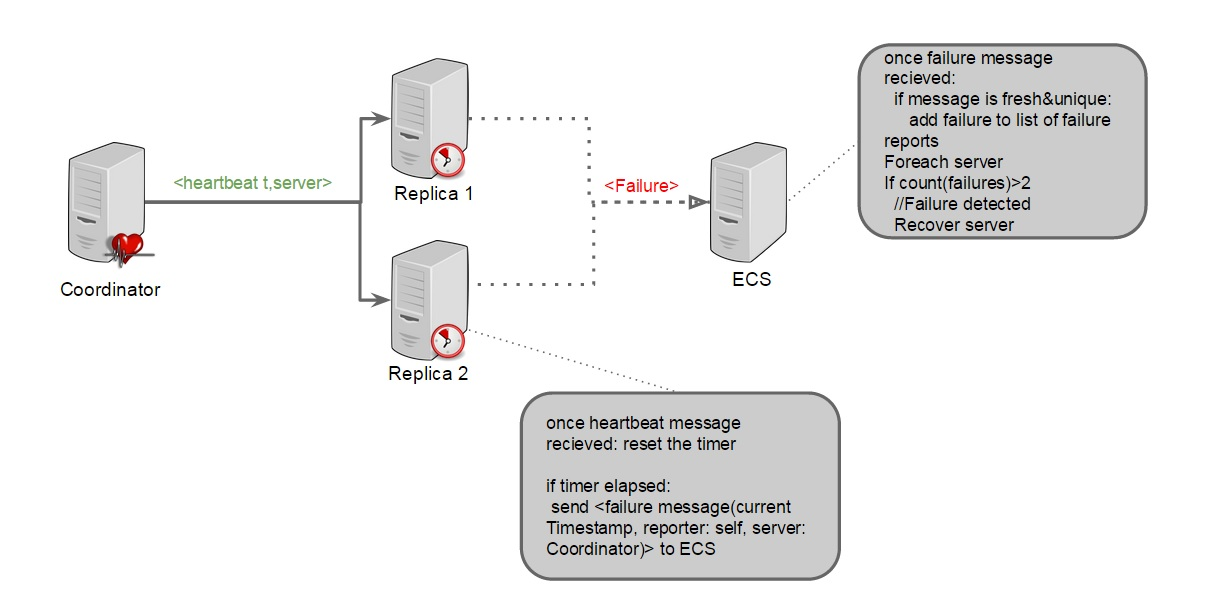
\includegraphics[width=0.5\textwidth]{FailureDetection.jpg}
\caption{Failure Detection Sketch \label{failuredetection}}
\end{figure}
\end{center}

\subsection{Extension}

\section{Implementation}
Key-value storage consists of three subsystems namely KVClient, KVServer, KVECS. 
To be elaborated ... @Arash @Ibrahim
\subsection{Client}
KVClient is the user intermediate layer in which the end-user with knowing only one server location can start using the cloud storage. KVClient application has following main features: \\
\textbf{connect} which allows the user to establish a connection to a server\\
\textbf{put} let user to store a key value pair in a server. In case that server is not responsible for demanded key the switching to the responsible server has been done automatically to ensure better user experience.\\
\textbf{get} user can query a key and like put command the responsibility of the servers has been encapsulated.\\
\textbf{gets} it retrieves the queried key by the user similar to get command. Plus to that, the client will be notified about the queried  key changes. In other words, by using this command user will be subscribed to the corresponding server. Therefore, Any value changes of the key by any client will lead to a push notification to the subscribed client.\\
\textbf{puts} It stores a key-value pair and subscribe to the key changes just like the gets.\\
\subsubsection{Subscription on client side}
For the subscription part we have implemented a separate thread to keep listening to the notification messages from the responsible servers. In case that new servers being added or removed from the system, the responsible server for each key might change due to the mapping constraints in the ring. To deal with responsibility changes, upon metadata updates on client side we subscribe all keys to corresponding servers. By this approach eventual consistency is guaranteed as well as no overhead on server side because clients are keeping track of their subscription.\\ 
On the server side, a list of subscribed servers per each key is being maintained and upon each put command the notifications are being published. For further details about the subscription feature refer to the server implementation details section \ref{serverimpl}.

\subsection{Server}\label{serverimpl}
to be added...
\subsection{ECS}
to be added...
\section{Evaluation}
to be added
\section{Discussion}
to be added
\section{Conclusion}
to be added

%ACKNOWLEDGMENTS are optional
\section{Acknowledgments}
To be added...
%
% The following two commands are all you need in the
% initial runs of your .tex file to
% produce the bibliography for the citations in your paper.
\bibliographystyle{abbrv}
\bibliography{sigproc}  % sigproc.bib is the name of the Bibliography in this case
% You must have a proper ".bib" file
%  and remember to run:
% latex bibtex latex latex
% to resolve all references
%
% ACM needs 'a single self-contained file'!
%
%APPENDICES are optional
%\balancecolumns

%\balancecolumns % GM June 2007
% That's all folks!
\end{document}
